%===========================================================================


\section{Model Performance: Internal Temporal Evaluation \texorpdfstring{[C]}{[C]}}
\label{sec:internal_performance}
%===========================================================================

Table~\ref{tab:internal_results} reports performance on the temporal test set
(2017--2019) under the unrestricted evaluation window.

\begin{table}[H]
    \centering\small
    \begin{tabular}{llrrrrr}
        \toprule
        \textbf{Var} & \textbf{Model}
        & \textbf{AUROC} & \textbf{AUPRC}
        & \textbf{Utility} & \textbf{Utility} & \textbf{Alert} \\
        & & & & \textbf{(0.5)} & \textbf{(best)} & \textbf{burden} \\
        \midrule
        A & Primary & \pcAurocPrimaryA & \pcAuprcPrimaryA & \pcUtilityPrimaryA & \pcUtilityMaxPrimaryA & \pcAlertBurdenPrimaryA \\
        A & GBT     & \pcAurocGbtA     & \pcAuprcGbtA     & \pcUtilityGbtA     & \pcUtilityMaxGbtA     & \pcAlertBurdenGbtA     \\
        A & NEWS2   & \pcAurocNewsA    & \pcAuprcNewsA    & \pcUtilityNewsA    & \pcUtilityMaxNewsA    & \pcAlertBurdenNewsA    \\
        A & Cox     & \pcAurocCoxA     & \pcAuprcCoxA     & \pcUtilityCoxA     & \pcUtilityMaxCoxA     & \pcAlertBurdenCoxA     \\
        A & qSOFA   & \pcAurocQsofaA   & \pcAuprcQsofaA   & \pcUtilityQsofaA   & \pcUtilityMaxQsofaA   & \pcAlertBurdenQsofaA   \\
        A & SIRS    & \pcAurocSirsA    & \pcAuprcSirsA    & \pcUtilitySirsA    & \pcUtilityMaxSirsA    & \pcAlertBurdenSirsA    \\
        \midrule
        B & Primary & \pcAurocPrimaryB & \pcAuprcPrimaryB & \pcUtilityPrimaryB & \pcUtilityMaxPrimaryB & \pcAlertBurdenPrimaryB \\
        B & GBT     & \pcAurocGbtB     & \pcAuprcGbtB     & \pcUtilityGbtB     & \pcUtilityMaxGbtB     & \pcAlertBurdenGbtB     \\
        B & NEWS2   & \pcAurocNewsB    & \pcAuprcNewsB    & \pcUtilityNewsB    & \pcUtilityMaxNewsB    & \pcAlertBurdenNewsB    \\
        B & Cox     & \pcAurocCoxB     & \pcAuprcCoxB     & \pcUtilityCoxB     & \pcUtilityMaxCoxB     & \pcAlertBurdenCoxB     \\
        B & qSOFA   & \pcAurocQsofaB   & \pcAuprcQsofaB   & \pcUtilityQsofaB   & \pcUtilityMaxQsofaB   & \pcAlertBurdenQsofaB   \\
        B & SIRS    & \pcAurocSirsB    & \pcAuprcSirsB    & \pcUtilitySirsB    & \pcUtilityMaxSirsB    & \pcAlertBurdenSirsB    \\
        \midrule
        C & Primary & \pcAurocPrimaryC & \pcAuprcPrimaryC & \pcUtilityPrimaryC & \pcUtilityMaxPrimaryC & \pcAlertBurdenPrimaryC \\
        C & GBT     & \pcAurocGbtC     & \pcAuprcGbtC     & \pcUtilityGbtC     & \pcUtilityMaxGbtC     & \pcAlertBurdenGbtC     \\
        C & NEWS2   & \pcAurocNewsC    & \pcAuprcNewsC    & \pcUtilityNewsC    & \pcUtilityMaxNewsC    & \pcAlertBurdenNewsC    \\
        C & Cox     & \pcAurocCoxC     & \pcAuprcCoxC     & \pcUtilityCoxC     & \pcUtilityMaxCoxC     & \pcAlertBurdenCoxC     \\
        C & qSOFA   & \pcAurocQsofaC   & \pcAuprcQsofaC   & \pcUtilityQsofaC   & \pcUtilityMaxQsofaC   & \pcAlertBurdenQsofaC   \\
        C & SIRS    & \pcAurocSirsC    & \pcAuprcSirsC    & \pcUtilitySirsC    & \pcUtilityMaxSirsC    & \pcAlertBurdenSirsC    \\
        \bottomrule
    \end{tabular}
    \caption{Internal temporal test performance (2017--2019, all variants use
    temporal split). N test rows: \pcNTestRowsB{} (B). \textbf{Utility (0.5)} is
    the normalised adapted PhysioNet-style Utility Score
    (Section~\ref{sec:metrics}) at the default cut-off;
    \textbf{Utility (best)} is its maximum over the threshold grid of
    Section~\ref{sec:metrics}. Zero is the no-alert strategy under both. Alert
    burden is at the 0.5 cut-off ($\infty$ = no true alerts there); the
    benchmark is 1.4 \cite{moor2023review}. Per-threshold curves are in
    Figure~\ref{fig:utility_sweep} and the attaining operating points in
    Table~\ref{tab:utility_optimum}. Confidence intervals for Variant B are in
    Table~\ref{tab:internal_ci}. \textbf{[C] confirmatory.}}
    \label{tab:internal_results}
\end{table}

\begin{table}[H]
    \centering\small
    \begin{tabular}{llll}
        \toprule
        \textbf{Model} & \textbf{AUROC} & \textbf{95\% CI} & \textbf{AUPRC (95\% CI)} \\
        \midrule
        Primary & \pcAurocPrimaryB & \pcAurocCiLoPrimaryB--\pcAurocCiHiPrimaryB & \pcAuprcPrimaryB{} \pcAuprcCiPrimaryB \\
        GBT     & \pcAurocGbtB     & \pcAurocCiLoGbtB--\pcAurocCiHiGbtB         & \pcAuprcGbtB{} \pcAuprcCiGbtB     \\
        NEWS2   & \pcAurocNewsB    & \pcAurocCiLoNewsB--\pcAurocCiHiNewsB       & \pcAuprcNewsB{} \pcAuprcCiNewsB    \\
        Cox     & \pcAurocCoxB     & \pcAurocCiLoCoxB--\pcAurocCiHiCoxB         & \pcAuprcCoxB{} \pcAuprcCiCoxB     \\
        qSOFA   & \pcAurocQsofaB   & \pcAurocCiLoQsofaB--\pcAurocCiHiQsofaB     & \pcAuprcQsofaB{} \pcAuprcCiQsofaB   \\
        SIRS    & \pcAurocSirsB    & \pcAurocCiLoSirsB--\pcAurocCiHiSirsB       & \pcAuprcSirsB{} \pcAuprcCiSirsB    \\
        \bottomrule
    \end{tabular}
    \caption{Variant B temporal test performance with 95\% stay-level
    cluster-bootstrap intervals ($B = 2{,}000$ replicates over
    \pcNTestRowsB{} test person-hours carrying \pcNTestEventsB{} sepsis onsets).
    These are \emph{marginal} intervals; paired differences are reported
    separately where claimed (H6, Section~\ref{sec:h6}). The primary model and
    GBT overlap almost completely, and both are separated from the other four
    models. \textbf{[C] confirmatory.}}
    \label{tab:internal_ci}
\end{table}

\subsection{Utility and Alert Burden Across Thresholds}
\label{sec:utility_threshold}

At the default 0.5 cut-off no model does better than issuing no alerts, but
this threshold is uninformative. The primary model scores \pcUtilityPrimaryB{}
under Variant B because its largest predicted hourly probability is far below
0.5, so it generates no alert. The models that do cross 0.5 (the rule-based
scores, rescaled onto the unit interval, and the Cox linear predictor) do so
so often that they score well below zero: \pcUtilityCoxB{} for Cox and
\pcUtilityQsofaB{} for qSOFA under Variant B. At this cut-off the models are
therefore separated by calibration rather than clinical value.

\begin{figure}[H]
    \centering
    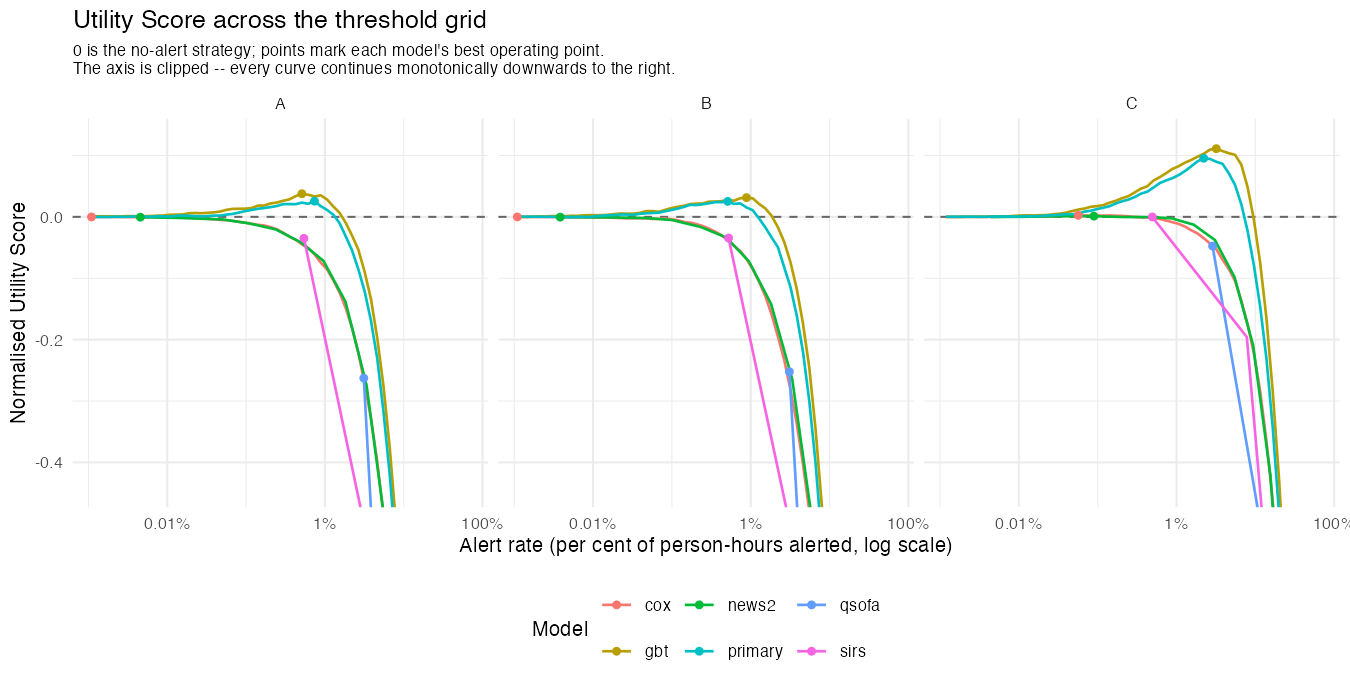
\includegraphics[width=\textwidth]{images/07_utility_threshold_sweep.png}
    \caption{Normalised Utility Score against alert rate for every model and
    pre-registered label variant on the temporal test set. The dashed line at
    zero is the no-alert strategy, and points mark each model's best operating
    point. Only the primary model and GBT rise above zero, peaking between 0.5
    and 3 per cent of person-hours alerted. The vertical axis is clipped; every
    curve falls to $-5$ or below at a 50 per cent alert rate.}
    \label{fig:utility_sweep}
\end{figure}

Figure~\ref{fig:utility_sweep} traces the whole threshold grid, and
Table~\ref{tab:utility_optimum} reports each model's best attainable score
together with the operating point that attains it.

\begin{table}[H]
    \centering\small
    \begin{tabular}{llrrrr}
        \toprule
        \textbf{Var} & \textbf{Model} & \textbf{Max utility}
        & \textbf{Alert rate} & \textbf{Stays} & \textbf{Alert} \\
        & & & \textbf{(\% p-h)} & \textbf{detected (\%)} & \textbf{burden} \\
        \midrule
        A & Primary & \pcUtilityMaxPrimaryA & \pcUtilityOptAlertPctPrimaryA & \pcUtilityOptDetectPctPrimaryA & \pcUtilityOptBurdenPrimaryA \\
        A & GBT     & \pcUtilityMaxGbtA     & \pcUtilityOptAlertPctGbtA     & \pcUtilityOptDetectPctGbtA     & \pcUtilityOptBurdenGbtA     \\
        A & NEWS2   & \pcUtilityMaxNewsA    & \pcUtilityOptAlertPctNewsA    & \pcUtilityOptDetectPctNewsA    & \pcUtilityOptBurdenNewsA    \\
        A & Cox     & \pcUtilityMaxCoxA     & \pcUtilityOptAlertPctCoxA     & \pcUtilityOptDetectPctCoxA     & \pcUtilityOptBurdenCoxA     \\
        A & qSOFA   & \pcUtilityMaxQsofaA   & \pcUtilityOptAlertPctQsofaA   & \pcUtilityOptDetectPctQsofaA   & \pcUtilityOptBurdenQsofaA   \\
        A & SIRS    & \pcUtilityMaxSirsA    & \pcUtilityOptAlertPctSirsA    & \pcUtilityOptDetectPctSirsA    & \pcUtilityOptBurdenSirsA    \\
        \midrule
        B & Primary & \pcUtilityMaxPrimaryB & \pcUtilityOptAlertPctPrimaryB & \pcUtilityOptDetectPctPrimaryB & \pcUtilityOptBurdenPrimaryB \\
        B & GBT     & \pcUtilityMaxGbtB     & \pcUtilityOptAlertPctGbtB     & \pcUtilityOptDetectPctGbtB     & \pcUtilityOptBurdenGbtB     \\
        B & NEWS2   & \pcUtilityMaxNewsB    & \pcUtilityOptAlertPctNewsB    & \pcUtilityOptDetectPctNewsB    & \pcUtilityOptBurdenNewsB    \\
        B & Cox     & \pcUtilityMaxCoxB     & \pcUtilityOptAlertPctCoxB     & \pcUtilityOptDetectPctCoxB     & \pcUtilityOptBurdenCoxB     \\
        B & qSOFA   & \pcUtilityMaxQsofaB   & \pcUtilityOptAlertPctQsofaB   & \pcUtilityOptDetectPctQsofaB   & \pcUtilityOptBurdenQsofaB   \\
        B & SIRS    & \pcUtilityMaxSirsB    & \pcUtilityOptAlertPctSirsB    & \pcUtilityOptDetectPctSirsB    & \pcUtilityOptBurdenSirsB    \\
        \midrule
        C & Primary & \pcUtilityMaxPrimaryC & \pcUtilityOptAlertPctPrimaryC & \pcUtilityOptDetectPctPrimaryC & \pcUtilityOptBurdenPrimaryC \\
        C & GBT     & \pcUtilityMaxGbtC     & \pcUtilityOptAlertPctGbtC     & \pcUtilityOptDetectPctGbtC     & \pcUtilityOptBurdenGbtC     \\
        C & NEWS2   & \pcUtilityMaxNewsC    & \pcUtilityOptAlertPctNewsC    & \pcUtilityOptDetectPctNewsC    & \pcUtilityOptBurdenNewsC    \\
        C & Cox     & \pcUtilityMaxCoxC     & \pcUtilityOptAlertPctCoxC     & \pcUtilityOptDetectPctCoxC     & \pcUtilityOptBurdenCoxC     \\
        C & qSOFA   & \pcUtilityMaxQsofaC   & \pcUtilityOptAlertPctQsofaC   & \pcUtilityOptDetectPctQsofaC   & \pcUtilityOptBurdenQsofaC   \\
        C & SIRS    & \pcUtilityMaxSirsC    & \pcUtilityOptAlertPctSirsC    & \pcUtilityOptDetectPctSirsC    & \pcUtilityOptBurdenSirsC    \\
        \bottomrule
    \end{tabular}
    \caption{Maximum achievable Utility Score and the operating point that
    attains it, over the sixty-point threshold grid, on the temporal test set.
    ``Alert rate'' is the percentage of test person-hours alerted; ``stays
    detected'' is the percentage of septic stays alerted within the reward
    window $[\text{onset}-6,\ \text{onset}]$; alert burden is false alerts per
    true alert at that same point, against the benchmark of 1.4
    \cite{moor2023review}; $\infty$ with a maximum at or below zero means the
    best strategy is to raise no alert. \textbf{[E] exploratory:} thresholds
    are chosen on the test set, so these are upper bounds on achievable
    utility.}
    \label{tab:utility_optimum}
\end{table}

After threshold sweeping, the two fitted models reach positive utility under
every variant. Under Variant B their maximum scores
are \pcUtilityMaxPrimaryB{} (primary) and \pcUtilityMaxGbtB{} (GBT), on a
scale bounded above by 1. These optima are attained at
\pcUtilityOptBurdenPrimaryB{} and \pcUtilityOptBurdenGbtB{} false alerts per
true alert, while detecting \pcUtilityOptDetectPctPrimaryB{} and
\pcUtilityOptDetectPctGbtB{} per cent of septic stays within the actionable
window. Under Variants A and B, NEWS2, Cox, qSOFA and SIRS have no threshold at
which alerting beats not alerting, and under Variant C their maxima do not
exceed \pcUtilityMaxCoxC. Across all variants, every positive maximum
is attained at between \pcUtilityOptBurdenPrimaryC{} and
\pcUtilityOptBurdenGbtB{} false alerts per true alert, twenty to thirty-seven
times the benchmark of 1.4 \cite{moor2023review}. The thresholds are selected
on the test set, so these values are optimistic upper bounds. AUROC values in
the mid-to-high 0.7s (Table~\ref{tab:internal_results}) therefore did not
translate into an operating point with a clinically plausible alert burden.

Decision-curve net benefit prices false alarms differently: at a threshold
matched to the event prevalence, the primary model achieves positive net
benefit over both default strategies (Table~\ref{tab:net_benefit},
Section~\ref{sec:clinical_utility}). This is an internal contrast between two
metrics, not a test of H5's internal-to-external estimand. Under both metrics,
no configuration tested approaches the alert-burden benchmark.

\subsection{Calibration \texorpdfstring{[C]}{[C]}}
\label{sec:calibration_results}

Calibration intercept and slope are two summary numbers describing a whole
curve, so both the curve itself and a scalar summary of its distance from the
diagonal are reported. Following Van Calster et al.\
\cite{vancalster2019calibration}, the flexible calibration curve is a
restricted cubic spline of the outcome on the logit of predicted risk, and it
is summarised by the Integrated Calibration Index (ICI, the mean absolute
distance between predicted risk and that curve) and the scaled Brier score,
$1 - \text{Brier}/\text{Brier}_{\text{null}}$, where the null model predicts
the prevalence for every person-hour.

\begin{table}[H]
    \centering\small
    \begin{tabular}{llrrrrr}
        \toprule
        \textbf{Var} & \textbf{Model} & \textbf{Intercept} & \textbf{Slope}
        & \textbf{ICI} & \textbf{$E_{\max}$} & \textbf{Scaled Brier} \\
        \midrule
        A & Primary & \pcCalibIntPrimaryA & \pcCalibSlopePrimaryA & \pcIciPrimaryA & \pcEmaxPrimaryA & \pcBrierScaledPrimaryA \\
        A & GBT     & \pcCalibIntGbtA     & \pcCalibSlopeGbtA     & \pcIciGbtA     & \pcEmaxGbtA     & \pcBrierScaledGbtA     \\
        A & Cox     & \pcCalibIntCoxA     & \pcCalibSlopeCoxA     & \pcIciCoxA     & \pcEmaxCoxA     & \pcBrierScaledCoxA     \\
        \midrule
        B & Primary & \pcCalibIntPrimaryB & \pcCalibSlopePrimaryB & \pcIciPrimaryB & \pcEmaxPrimaryB & \pcBrierScaledPrimaryB \\
        B & GBT     & \pcCalibIntGbtB     & \pcCalibSlopeGbtB     & \pcIciGbtB     & \pcEmaxGbtB     & \pcBrierScaledGbtB     \\
        B & Cox     & \pcCalibIntCoxB     & \pcCalibSlopeCoxB     & \pcIciCoxB     & \pcEmaxCoxB     & \pcBrierScaledCoxB     \\
        \midrule
        C & Primary & \pcCalibIntPrimaryC & \pcCalibSlopePrimaryC & \pcIciPrimaryC & \pcEmaxPrimaryC & \pcBrierScaledPrimaryC \\
        C & GBT     & \pcCalibIntGbtC     & \pcCalibSlopeGbtC     & \pcIciGbtC     & \pcEmaxGbtC     & \pcBrierScaledGbtC     \\
        C & Cox     & \pcCalibIntCoxC     & \pcCalibSlopeCoxC     & \pcIciCoxC     & \pcEmaxCoxC     & \pcBrierScaledCoxC     \\
        \bottomrule
    \end{tabular}
    \caption{Calibration on the temporal test set. Perfect calibration is
    intercept = 0, slope = 1, ICI = 0. A scaled Brier score at or below zero
    means the model is no better than predicting the prevalence for everyone.
    NEWS2, qSOFA and SIRS are omitted: their score-to-probability lookups take
    only \pcNDistinctNews, \pcNDistinctQsofa{} and \pcNDistinctSirs{} distinct
    values respectively, too few to support a flexible calibration curve.}
    \label{tab:calibration}
\end{table}

The primary model is the only evaluated model whose predicted probabilities
stay close to observed risks, under every label variant: its intercept sits
within \pcCalibIntMaxAbsPrimary{} of zero, its slope within
\pcCalibSlopeMaxDevPrimary{} of one
(\pcCalibSlopePrimaryA, \pcCalibSlopePrimaryB, \pcCalibSlopePrimaryC), and its
largest ICI across the three variants is \pcIciPrimaryC{}, under a fifth of
the 0.2 per cent event rate.
Its scaled Brier score is positive under all three, though barely
(\pcBrierScaledPrimaryA{} to \pcBrierScaledPrimaryC), meaning it improves on
the null model by less than one per cent.

\paragraph{Intervals on intercept and slope.} Protocol Amendment 10 attaches
intervals to these two quantities, which at \pcNTestRowsB{} person-hours are
narrow. The slope covers one under the
Narrow and Standard variants (\pcCalibSlopeCiA{} and \pcCalibSlopeCiB) but not
under the Liberal one (\pcCalibSlopeCiC); the intercept covers zero under the
Liberal variant (\pcCalibIntCiC) but not under the other two
(\pcCalibIntCiA{} and \pcCalibIntCiB). Under each variant one of the two
absolute targets is therefore missed at this confidence: the miscalibration is
statistically detectable but small. An intercept of \pcCalibIntPrimaryB{} on
the logit scale at an event rate of \pcPrevalenceB{} moves the predicted hourly
risk by about a tenth of itself and moves no operating point on the threshold
grid of Section~\ref{sec:clinical_utility}.

GBT and Cox are severely miscalibrated, with intercepts near $-6$ and strongly
negative scaled Brier scores. The Variant B GBT scaled Brier score of
\pcBrierScaledGbtB{}, for example, indicates a squared error
\pcBrierRatioGbtB{} times that of predicting the prevalence for every
person-hour. GBT emits predicted risks between 0.2 and 0.9 for person-hours
whose observed event rate never exceeds 0.04 (Figure~\ref{fig:calibration}),
so its best operating point, near \pcUtilityOptThresholdGbtB{} under Variant B
(Table~\ref{tab:utility_optimum}), can be located only empirically and has no
interpretation as a risk.

Across variants, slopes of \pcCalibSlopePrimaryA, \pcCalibSlopePrimaryB{} and
\pcCalibSlopePrimaryC{} sit within \pcCalibSlopeSpread{} of one another, and
the paired cross-label contrasts against the primary label are
\pcCalibDeltaSlopeAB{} [\pcCalibDeltaSlopeCiLoAB, \pcCalibDeltaSlopeCiHiAB]
for the Narrow variant and \pcCalibDeltaSlopeCB{}
[\pcCalibDeltaSlopeCiLoCB, \pcCalibDeltaSlopeCiHiCB] for the Liberal one:
both intervals cover zero, so the label is not shown to change the calibration
slope. The Liberal-against-Standard \emph{intercept} contrast, by contrast, is
\pcCalibDeltaIntCB{} [\pcCalibDeltaIntCiLoCB, \pcCalibDeltaIntCiHiCB], which
excludes zero; the displacement is small on the probability scale at a
\pcPrevalenceB{} event rate. The label definition therefore shifts the
calibration intercept slightly but is not shown to change the slope.

\begin{figure}[H]
    \centering
    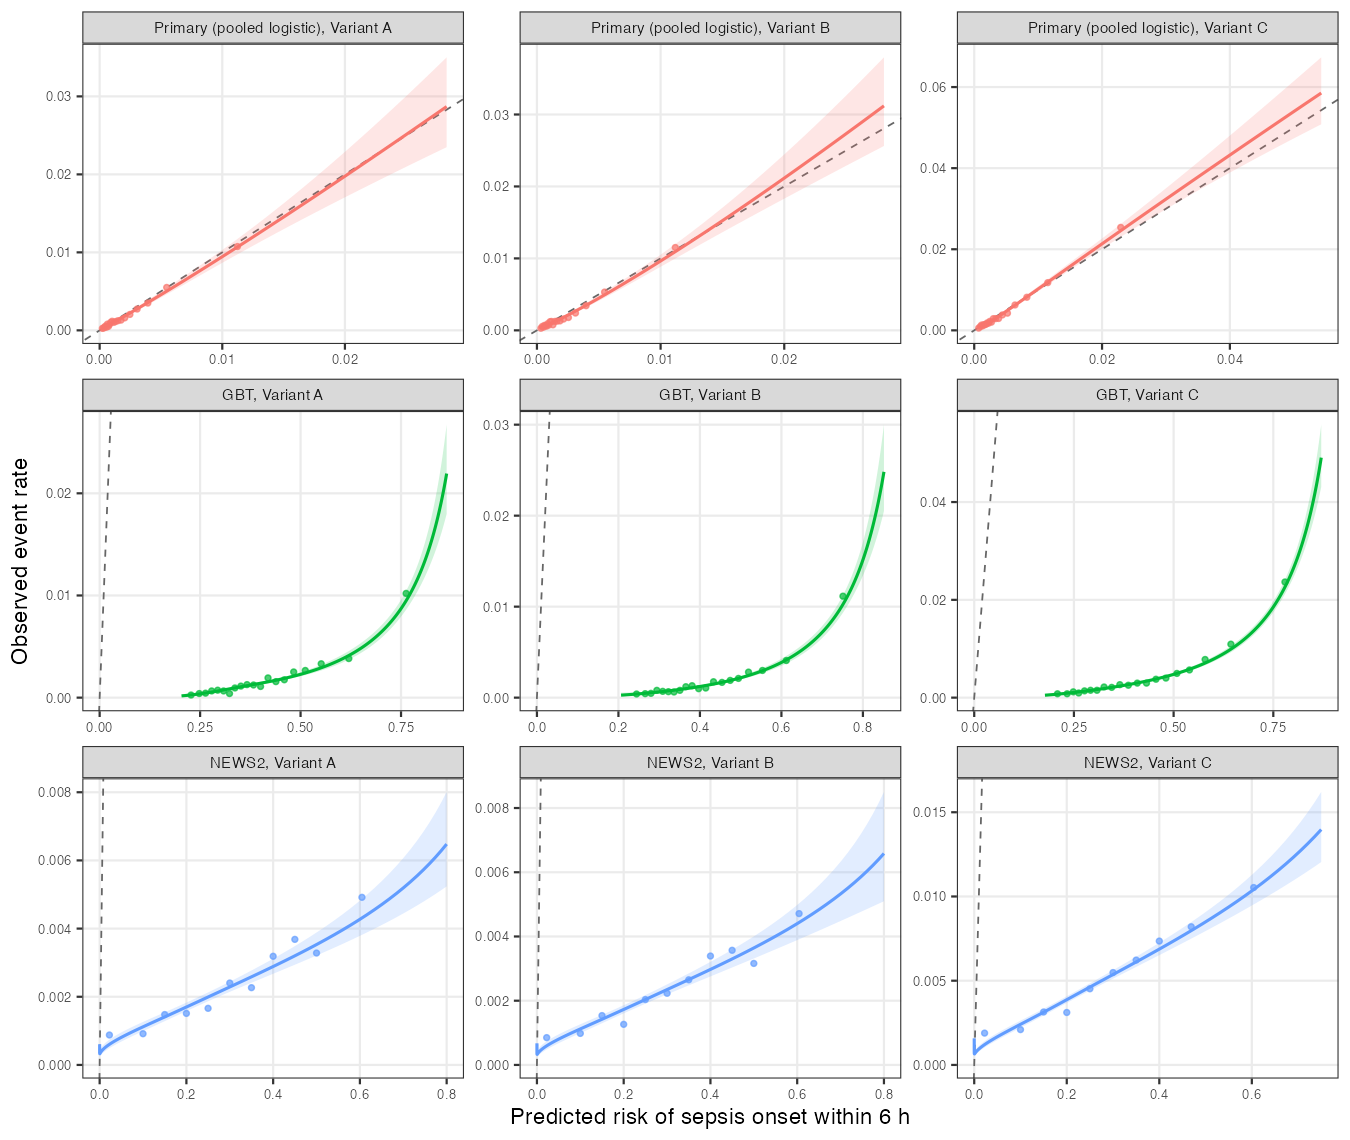
\includegraphics[width=\textwidth]{images/11_calibration_curves.png}
    \caption{Flexible calibration curves on the temporal test set. Dashed line
    = perfect calibration; points = twenty equal-sized bins of predicted risk;
    shaded band = 95\% confidence interval. Each panel has its own scale
    because the predicted-risk ranges differ by orders of magnitude.}
    \label{fig:calibration}
\end{figure}

\subsubsection{Sensitivity to the Probability Clamp}

Calibration is often computed after clamping predicted probabilities to
$[0.001, 0.999]$. That guard is standard for models whose predictions approach
0 or 1, but at a 0.2 per cent hourly event rate it distorts the estimate:
\pcPctBelowClampPrimaryA\% (Variant A),
\pcPctBelowClampPrimaryB\% (Variant B) and \pcPctBelowClampPrimaryC\%
(Variant C) of the primary model's predicted probabilities fall \emph{below}
the clamp floor, so the clamp overwrites a large share of the quantity being
measured. No predicted probability exceeds \pcMaxPredPrimaryC{} under any
variant, so only the floor binds. The values in Table~\ref{tab:calibration}
use a floor of $10^{-6}$. Under the conventional clamp the primary model's Variant A slope is
\pcCalibSlopeClampedPrimaryA{}, against \pcCalibSlopePrimaryA{} on the
$10^{-6}$ floor, so a calibration guard chosen without reference to the event
rate itself changes the reported estimate.
